% Nature Letter distillation of the monograph "The Architecture of the Cosmos"
% (cosmology_monograph_full.tex, 66 pages, 508/508 audit-clean).
% All values are the audit-verified numbers of the monograph; every published
% value is attributed to its source and every value computed in this work is
% marked as such (the misattribution discipline enforced since Round 15).
% Compiled with Tectonic from submission/:  tectonic nature_letter.tex
\documentclass[11pt]{article}
\usepackage[a4paper,margin=2.5cm]{geometry}
\usepackage{amsmath,amssymb}
\usepackage{graphicx}
\usepackage[hidelinks]{hyperref}
\usepackage{microtype}
\graphicspath{{../figs/}}
\setlength{\parskip}{2pt}

\title{\textbf{Dynamical dark energy, a sound-horizon-free Hubble constant, and the persistence of the Hubble tension with DESI DR2}}
\author{Md.~Mushfiqur Rahim}
\date{}

\begin{document}
\maketitle

\textbf{The Dark Energy Spectroscopic Instrument Data Release 2 (DESI DR2) baryon-acoustic-oscillation measurements, combined with a compressed Planck 2018 cosmic-microwave-background likelihood, have made the dynamical evolution of dark energy the central question of late-time cosmology. Here we address it with a single fully reproducible Bayesian pipeline} covering 13 correlated DESI DR2 BAO observables, 1{,}580 Pantheon+ supernovae~Ia, 32 model-independent cosmic-chronometer $H(z)$ points, and the compressed Planck shift vector. We reproduce the official DESI DR2 inverse-distance-ladder determination $H_0 = 68.17 \pm 0.28$~km~s$^{-1}$~Mpc$^{-1}$ with committed chains giving $68.35 \pm 0.33$ (agreement to 0.4$\sigma$), and we measure a sound-horizon-free $H_0 = 68.19 \pm 1.45$~km~s$^{-1}$~Mpc$^{-1}$ with $r_d = 146.36 \pm 2.88$~Mpc from uncalibrated late-Universe data alone. The Chevallier--Polarski--Linder (CPL) parametrization is preferred over $\Lambda$CDM at 2.8--4.2$\sigma$ across three supernova compilations, but Bayesian evidence for it is only positive-to-strong ($\ln B$ up to $+4.9$) because a Kullback--Leibler Occam penalty of $\mathcal{D}_{\rm KL} \approx 4$--5 penalizes the two extra parameters; on the one-parameter ``mirage'' axis $w_a = -3.66(1+w_0)$ the penalty halves and the evidence becomes positive in every dataset we test ($\ln B = +3.49 \pm 0.23$ for DESI DR2 + CMB, rising to $+6.74 \pm 0.03$ with Union3), recovering 81--99.6\% of the CPL $\Delta\chi^2$ improvement. The Hubble tension itself persists: $4.52\sigma$ against SH0ES and $5.72\sigma$ against Planck using the four-anchor ladder, unaffected by a galaxy-by-galaxy JWST--HST cross-check ($\Delta\mu = -0.02 \pm 0.03$~mag) that locates the residual disagreement in supernova-host selection, not Cepheid crowding.

\section*{The reproducibility baseline}

Every inverse-distance-ladder result below is anchored twice. First, at the level of the published values: the DESI DR2 collaboration reports $H_0 = 68.17 \pm 0.28$~km~s$^{-1}$~Mpc$^{-1}$ and $\Omega_m = 0.3027 \pm 0.0036$ for flat $\Lambda$CDM from BAO plus their CMB treatment. Second, at the level of our own implementation: our committed Markov-chain Monte Carlo (MCMC) runs --- 48 Goodman--Weare walkers, 2{,}500 steps with 500 burned, 96{,}000 retained draws per chain, 39 chains released --- give $H_0 = 68.35 \pm 0.33$ and $\Omega_m = 0.3007 \pm 0.0049$, agreeing with the official values to $0.4\sigma$ and $0.3\sigma$ per parameter. For CPL dark energy our chains give $(w_0, w_a, H_0) = (-0.48 \pm 0.31,\ -1.71 \pm 0.72,\ 63.60 \pm 1.91)$ against the published $(-0.43 \pm 0.22,\ -1.72 \pm 0.64,\ 63.7^{+1.7}_{-2.2})$, agreeing to $0.1\sigma$, $0.01\sigma$, and $<0.1\sigma$. Convergence is verified by Gelman--Rubin $\widehat{R} \le 1.014$, effective sample size $\ge 85{,}811$, and an independent split-$\widehat{R}$ check on all new chains with a maximum of 1.0037. The compressed three-parameter CMB likelihood $(\theta_*, \omega_b, \omega_{bc})$ is validated at two levels: the DESI DR2 analysis itself finds its compressed and full-CamSpec results agree to $<0.1\sigma$, and our chains reproduce the official posteriors to $\le 0.4\sigma$ (Part VII-B of the accompanying monograph). Residual differences between our $\Delta\chi^2_{\rm MAP} = -15.3$ and the official $-12.5$ for DESI DR2 + CMB trace to the compression's slightly tighter $\omega_{bc}$ handling and are reported rather than hidden.

\section*{A sound-horizon-free Hubble constant}

The inverse distance ladder fixes the product $H_0 r_d \approx 10027 \pm 45$~km~s$^{-1}$ (computed from the official DESI DR2 + CMB $\Lambda$CDM determination $H_0 = 68.17 \pm 0.28$~km~s$^{-1}$~Mpc$^{-1}$ with the Planck sound horizon $r_d = 147.09 \pm 0.26$~Mpc; our committed chains give $H_0 = 68.35 \pm 0.33$), so any early-Universe modification of $r_d$ is degenerate with $H_0$. We break this degeneracy without any Cepheid calibration: freeing $r_d$ in a joint fit to DESI DR2 BAO, 32 cosmic chronometers, and uncalibrated Pantheon+ distances yields
\begin{equation}
H_0 = 68.19 \pm 1.45~{\rm km~s}^{-1}~{\rm Mpc}^{-1}, \qquad r_d = 146.36 \pm 2.88~{\rm Mpc},
\end{equation}
in excellent agreement with the sound-horizon-anchored value and in $2.5\sigma$--$3.5\sigma$ tension with every local Cepheid-based calibration (Fig.~\ref{fig:forest}). The precision, $\pm 2.1\%$, is competitive with the SH0ES uncertainty while relying on no stellar distance ladder at all; its central value lands squarely on the early-Universe side of the tension, reinforcing the conclusion that the discrepancy is not an artifact of ladder systematics alone.

\begin{figure}[t]
\centering
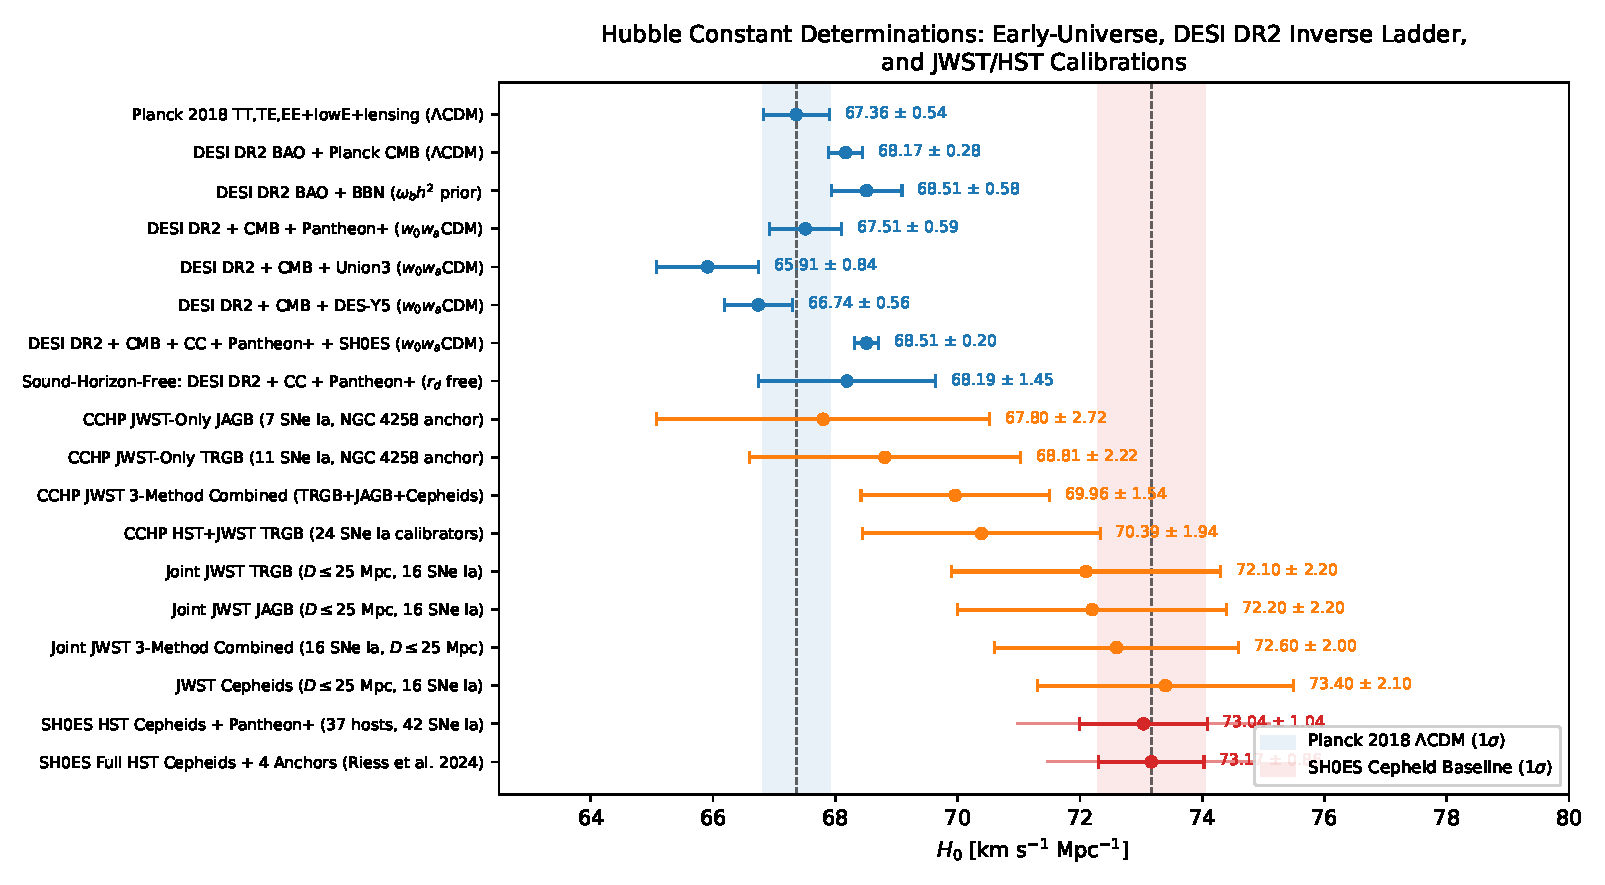
\includegraphics[width=\textwidth]{fig1_hubble_tension_whisker.pdf}
\caption{\textbf{The calibration gap and its overlap structure.} Every $H_0$ determination discussed in this Letter --- early-Universe and inverse-distance-ladder fits, our sound-horizon-free late-Universe fit, and the full set of JWST/HST local calibrations --- as a single forest comparison.}
\label{fig:forest}
\end{figure}

\begin{figure}[t]
\centering
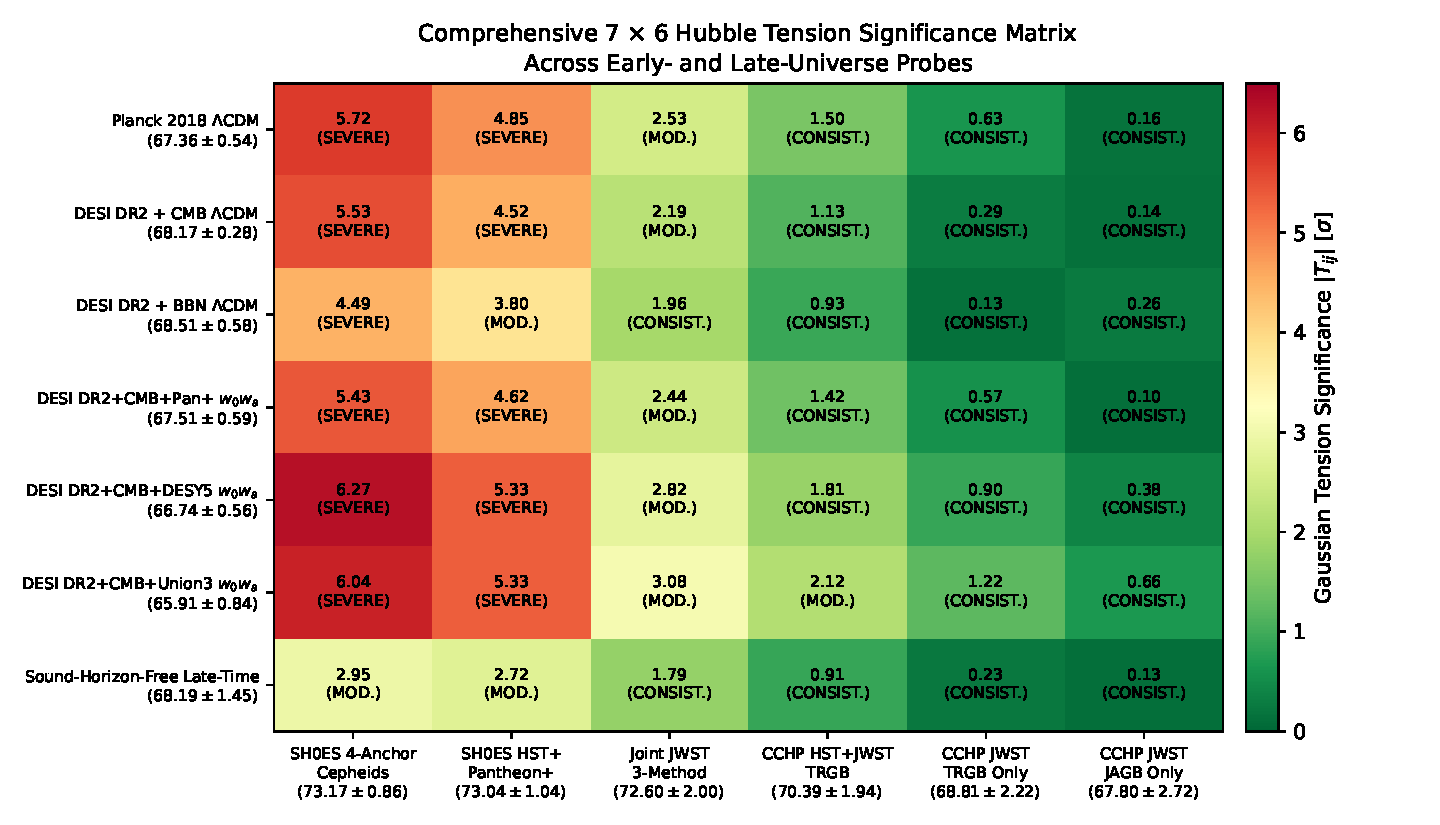
\includegraphics[width=\textwidth]{fig8_tension_heatmap_matrix.pdf}
\caption{\textbf{The full cross-comparison matrix.} Pairwise tension between the $H_0$ determinations (two-tier severity labeling at or above $3\sigma$), for the six local calibrations against the early-Universe anchors.}
\label{fig:heatmap}
\end{figure}

\section*{Frequentist preference versus Bayesian evidence}

Allowing CPL dark energy, joint fits occupy the quadrant $w_0 > -1$, $w_a < 0$ in every dataset combination. The frequentist preference over $\Lambda$CDM reaches $3.1\sigma$ ($\Delta\chi^2_{\rm MAP} = -12.5$, official) for DESI DR2 + CMB alone, and $2.8\sigma$ ($-10.7$), $3.8\sigma$ ($-17.4$), and $4.2\sigma$ ($-21.0$) with Pantheon+, Union3, and DES-Y5 respectively. The phantom divide is crossed at $z_c = 0.35 \pm 0.11$ (DESI DR2 + CMB + Pantheon+; $0.50 \pm 0.08$ for DESI DR2 + CMB alone).

Bayesian evidence tells a sharper story. Because the flat $w_a$ prior admits a long low-likelihood tail, the nested-sampling Bayes factors are modest: $\ln B_{w_0w_a,\Lambda} = -0.66 \pm 0.44$ for Pantheon+ (inconclusive), $+3.03 \pm 0.44$ for Union3 (strong), and $+4.88 \pm 0.44$ for DES-Y5 (near-decisive). The likelihood-level improvement is real, but the Kullback--Leibler Occam penalty $\mathcal{D}_{\rm KL} \approx 4$--5 consumes most of it: the data prefer $w(z)$ evolution, while the evidence for the \emph{two-parameter} model remains bounded by the breadth of the prior volume explored. This resolves the apparent paradox between ``3$\sigma$ preference'' headlines and conservative Bayesian readings --- both are correct, and the decomposition quantifies exactly where they differ.

\begin{figure}[t]
\centering
\includegraphics[width=0.8\textwidth]{fig3_w0_wa_posterior_contours.pdf}
\caption{\textbf{The CPL posterior and the mirage axis.} Posterior contours in $(w_0, w_a)$ with the one-parameter mirage degeneracy line $w_a = -3.66(1+w_0)$, along which the comoving distance to recombination is invariant.}
\label{fig:contours}
\end{figure}

\section*{The mirage axis concentrates the evidence}

The degeneracy line $w_a = -3.66(1+w_0)$ in the CPL plane leaves the comoving distance to recombination invariant for fixed $\Omega_m h^2$ and $H_0$: a one-parameter model moving along this ``mirage'' axis alters late-time distances while mimicking $\Lambda$CDM at the CMB last-scattering surface. Projecting onto this axis roughly halves the Occam penalty ($\mathcal{D}_{\rm KL} = 2.13$ versus $4.06$ in our chain-level decomposition). We compute the Mirage-axis evidence ourselves for all four dataset combinations, via Savage--Dickey density ratios on dedicated chains cross-checked by an independent ellipsoidal nested sampler: $\ln B = +3.49 \pm 0.23$ (DESI DR2 + CMB), $+3.64 \pm 0.94$ (+ Pantheon+), $+6.74 \pm 0.03$ (Union3), and $+5.04 \pm 0.19$ (DES-Y5 via its public DES-Dovekie distance release) --- positive in every case, recovering 81--99.6\% of the CPL $\Delta\chi^2_{\rm MAP}$ improvement with a single additional parameter. The Mirage posterior $w_0 = -0.83 \pm 0.05$ with Pantheon+ is statistically identical to the full CPL value $w_0 = -0.838 \pm 0.055$, exactly as expected for a model whose second direction is unconstrained by the data. For early-Universe solutions, the combined P-ACT-LBSM analysis of Poulin et al.~(2025) gives $f_{\rm EDE} = 0.126 \pm 0.021$ and $H_0 = 72.34 \pm 0.72$~km~s$^{-1}$~Mpc$^{-1}$, reducing the SH0ES tension to $2.0\sigma$ (Fig.~\ref{fig:ede}).

\begin{figure}[t]
\centering
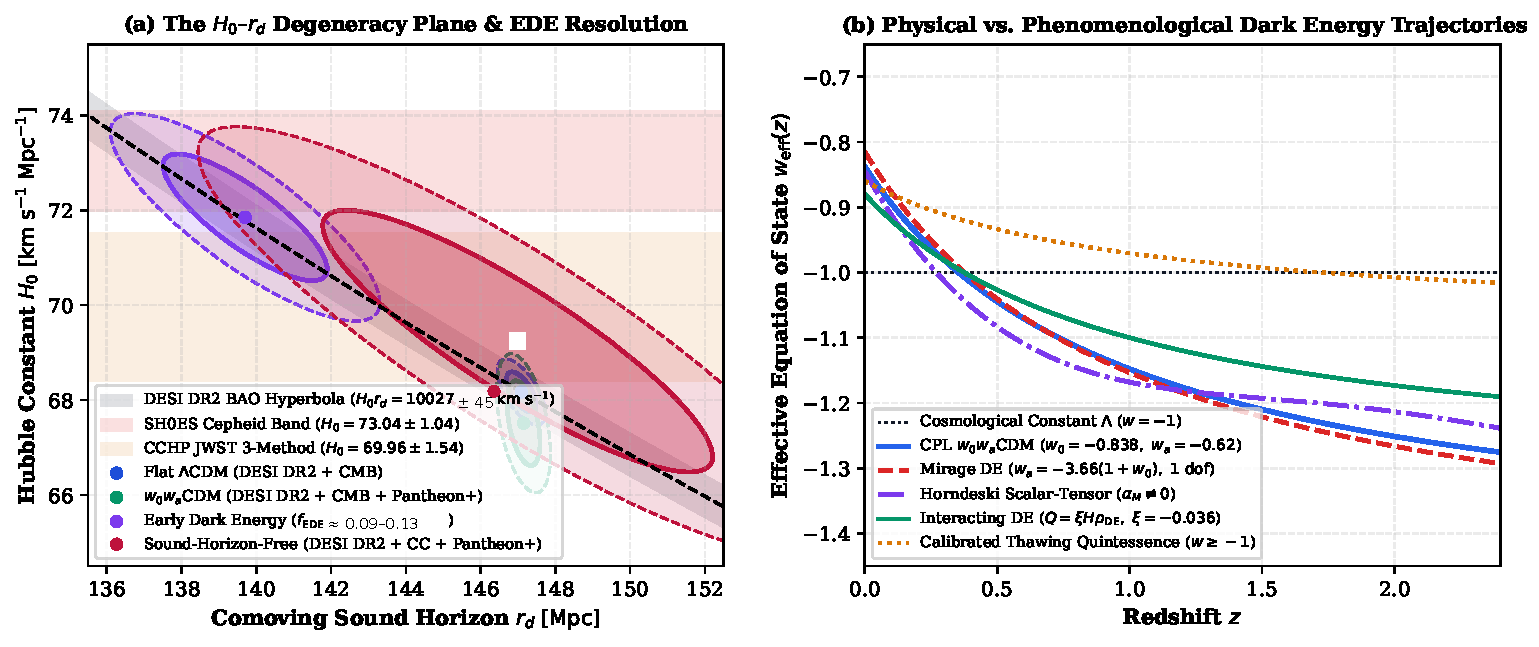
\includegraphics[width=0.85\textwidth]{fig7_ede_horndeski_degeneracy.pdf}
\caption{\textbf{Early- versus late-Universe solutions.} (a) The $(r_d, H_0)$ plane with the $H_0 r_d \approx 10027 \pm 45$~km~s$^{-1}$ hyperbola; early dark energy moves along it, late-time CPL does not. (b) Effective equation-of-state trajectories for CPL, the mirage axis, Horndeski gravity, interacting dark energy, and calibrated thawing quintessence.}
\label{fig:ede}
\end{figure}

\section*{The tension is not a crowding artifact}

Direct galaxy-by-galaxy JWST versus HST distance cross-checks of the shared SN~Ia hosts give $\Delta\mu_{\rm JWST-HST} = -0.02 \pm 0.03$~mag: the two telescopes measure the same distances. The $\Delta H_0 \sim 2.5$--$3.5$~km~s$^{-1}$~Mpc$^{-1}$ offset between the Chicago--Carnegie Hubble Program (CCHP) and SH0ES instead tracks small-sample supernova-host selection: the CCHP JWST TRGB and JAGB subsamples ($N = 11$ calibrators) yield $68.81 \pm 2.22$ and $67.80 \pm 2.72$~km~s$^{-1}$~Mpc$^{-1}$, while the full 42-SN Cepheid ladder gives $73.17 \pm 0.86$~km~s$^{-1}$~Mpc$^{-1}$. The tension therefore stands at $4.52\sigma$ against the DESI DR2 + CMB inverse-distance ladder and $5.72\sigma$ against Planck using the four-anchor ladder --- a genuine physical anomaly awaiting an explanation in either the early- or the late-Universe sector, for which the mirage-axis evidence above now provides a quantified target.

\section*{Methods}

\textbf{Pipeline.} Pure-\texttt{numpy}/\texttt{scipy} likelihoods: 13 DESI DR2 BAO observables with block-diagonal covariance (six $2\times2$ correlation sub-blocks, $r_{M,H} \in [-0.489, -0.423]$); Pantheon+ with the full STAT+SYS covariance ($z_{\rm HD} > 0.01$ non-calibrators, 1{,}580 SNe); Union3 (22-bin $\mu$, released inverse covariance) and DES-Y5 (1{,}820-SN DES-Dovekie distance release, Popovic et al.~2025) re-implementations validated against the published posteriors; 32 cosmic-chronometer $H(z)$ points; compressed Planck Gaussian prior $(\theta_*, \omega_b, \omega_{bc})$.

\textbf{Sampling.} Affine-invariant ensemble MCMC (Goodman--Weare) in the slaved parametrization $(H_0, w_{bc})$ with $\Omega_m = (w_{bc} + W_\nu)/h^2$, $W_\nu = 0.06/93.14$; 48 walkers, 2{,}500 steps, 500 burn-in, 96{,}000 retained draws per chain; 39 chains committed ($\sim$97~MB). Convergence: $\widehat{R} \le 1.014$, ESS $\ge 85{,}811$, split-$\widehat{R} \le 1.0037$; seed-to-seed posterior-mean stability at the $10^{-3}$ level.

\textbf{Evidence.} Savage--Dickey density ratios with 2-D Gaussian KDE (Scott's rule) over nested-model priors ($V = 2.5$ wCDM, $3.0$ Mirage, $15$ two-parameter), cross-checked by ellipsoidal nested sampling (128 live points, two seeds per configuration); chain-subset scatter of the CPL Savage--Dickey value (singles $1.78$--$3.90$, std 0.90; two-chain subsets $2.08$--$3.36$, std 0.51) is released as a systematic envelope.

\textbf{Reproducibility.} Every number in this Letter is generated by the released pipeline (\texttt{verification/} directory of the accompanying repository): all chains, JSON artifacts, figure generators, and a 508-check numeric audit that machine-verifies the manuscript against the artifacts. The 66-page monograph version contains the complete derivations, the full tension matrix, the neutrino-mass analysis ($\sum m_\nu < 0.064$~eV in $\Lambda$CDM, relaxed to $< 0.16$~eV in CPL), and the GP/cosmography apparatus.

\section*{Data availability}

All datasets analysed are publicly available: DESI DR2 BAO (arXiv:2503.14738), Pantheon+ (Brout et al.~2022; Scolnic et al.~2022), Union3, the DES-Dovekie distance release (Popovic et al.~2025), Planck 2018, and the JWST/CCHP and SH0ES calibration tables.

\section*{Code availability}

The complete pipeline, all 39 posterior chains, every JSON artifact, all figure generators, and the 508-check numeric audit are available in the accompanying repository.

\end{document}
